\section{Adjusting the queuing model}\label{sec:scenarios}

With the queuing model established and validated in
Section~\ref{sec:wasserstein}, an investigation into the parameters of the model
can be conducted. This section is comprised of several `what-if' scenarios --- a
classic component of healthcare operational research --- under this novel
parameterisation. The outcomes of interest in this work are server (resource)
utilisation and system times as these capture the both the driving forces of
cost and the overall state of the system. Specifically, the objective of these
experiments is to address the following questions:
\begin{itemize}
    \item How would the system be affected by a change in overall patient
        arrivals?
    \item How is the system affected by a change in resource availability (i.e.\
        a change in \(c\))?
    \item How is the system affected by patients moving between clusters?
\end{itemize}

Owing to the nature of the observed data, the queuing model parameterisation
and its assumptions, the effects of each scenario are given in relative terms
with respect to the base case. The base case being those results generated from
the best parameter set found in Section~\ref{sec:model}.

As mentioned in Section~\ref{sec:intro}, the source code used throughout this
work is available online and has been archived. %TODO Add citation for repo
In addition to this, the datasets generated from the simulations in this section
have been archived. %TODO archive and add citation


\subsection{Changes to overall patient arrivals}\label{subsec:arrivals}

Changes in overall patient arrivals to a queue reflect real-world scenarios
where some stimulus is improving (or worsening) the condition of the patient
population. Examples of positive stimuli include increased community care and
campaigns against harmful behaviours such as smoking. Within this model, overall
patient arrivals are altered using a scaling factor denoted by
\(\sigma\in\mathbb{R}\). This scaling factor is applied to the model by
multiplying each cluster's arrival rate by \(\sigma\). That is, for cluster
\(i\), its new arrival rate, \(\hat\lambda_i\), is given by:
\begin{equation}\label{eq:lambda}
    \hat\lambda_{i} = \sigma\lambda_i
\end{equation}

\begin{figure}
    \centering
    \begin{subfigure}{.5\imgwidth}
        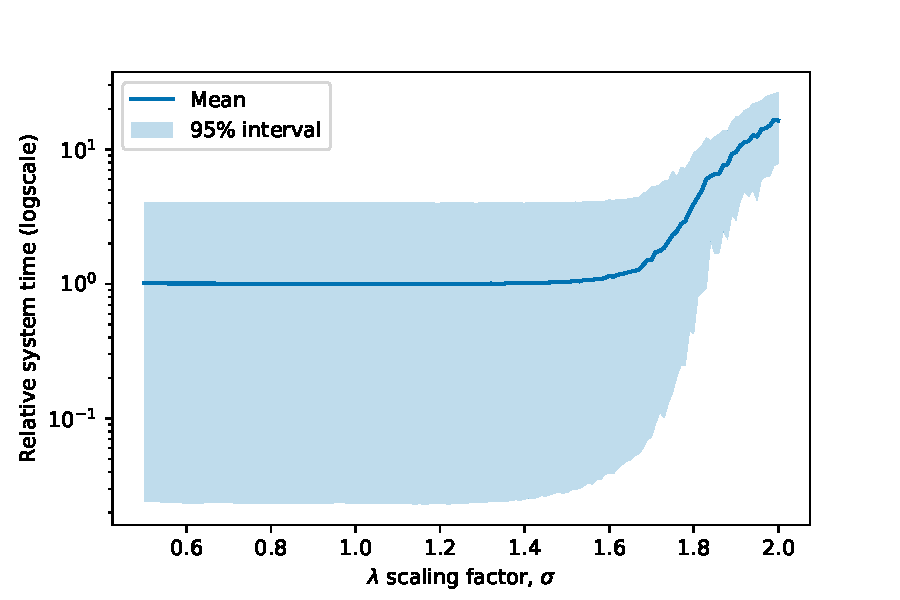
\includegraphics[width=\linewidth]{lambda_time}
        \caption{}\label{fig:lambda_time}
    \end{subfigure}\hfill%
    \begin{subfigure}{.5\imgwidth}
        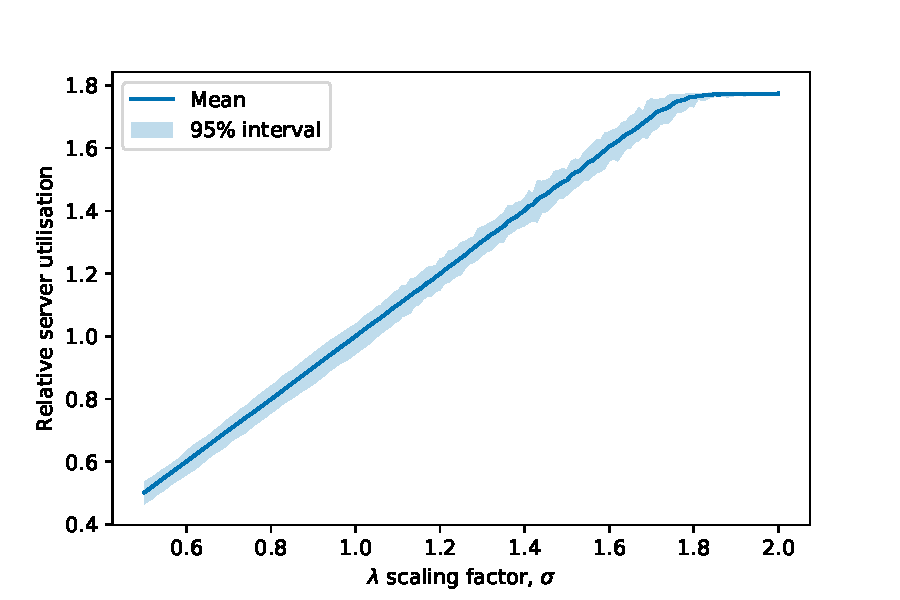
\includegraphics[width=\linewidth]{lambda_utilisation}
        \caption{}\label{fig:lambda_utilisation}
    \end{subfigure}
    \caption{%
        Plots of \(\sigma\) against relative (\subref{fig:lambda_time}) system
        time and (\subref{fig:lambda_utilisation}) mean server utilisation.
    }\label{fig:lambda}
\end{figure}


\subsection{Changes to resource availability}\label{subsec:resources}

\begin{figure}
    \centering
    \begin{subfigure}{.5\imgwidth}
        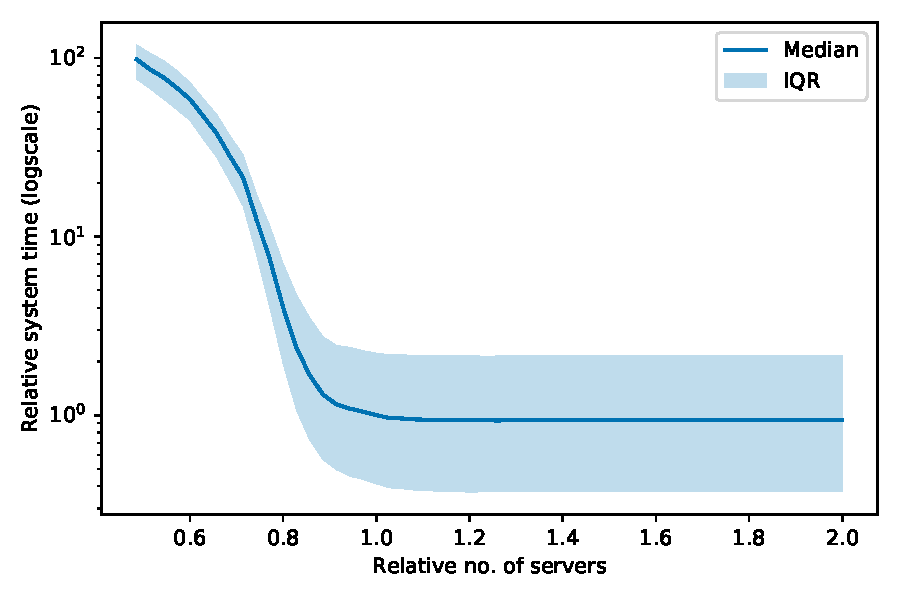
\includegraphics[width=\linewidth]{servers_time}
        \caption{}\label{fig:servers_time}
    \end{subfigure}\hfill%
    \begin{subfigure}{.5\imgwidth}
        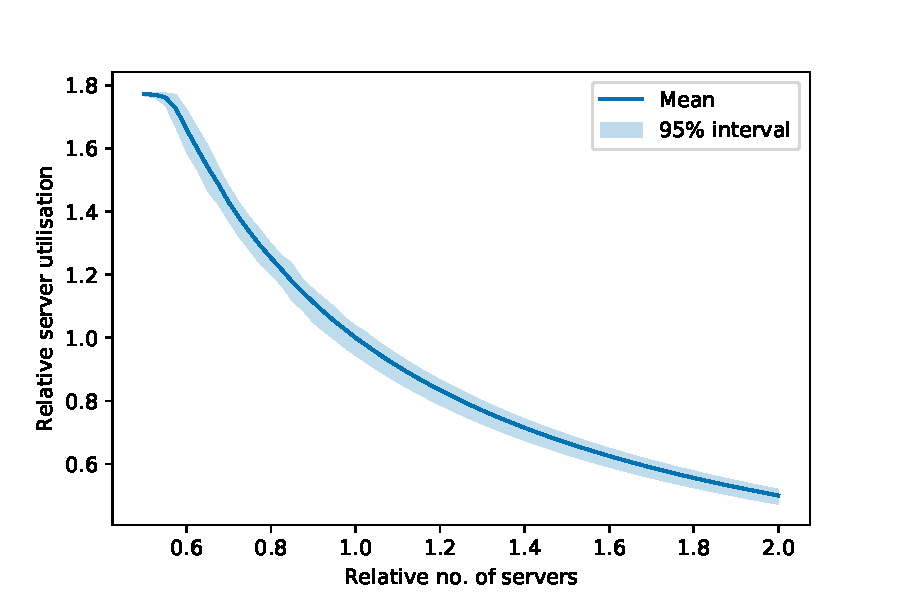
\includegraphics[width=\linewidth]{servers_utilisation}
        \caption{}\label{fig:servers_utilisation}
    \end{subfigure}
    \caption{%
        Plots of the relative number of servers against relative
        (\subref{fig:servers_time}) system time and
        (\subref{fig:servers_utilisation}) mean server utilisation.
    }
\end{figure}


\subsection{Moving patients between clusters}\label{subsec:moving}

\begin{figure}
    \centering
    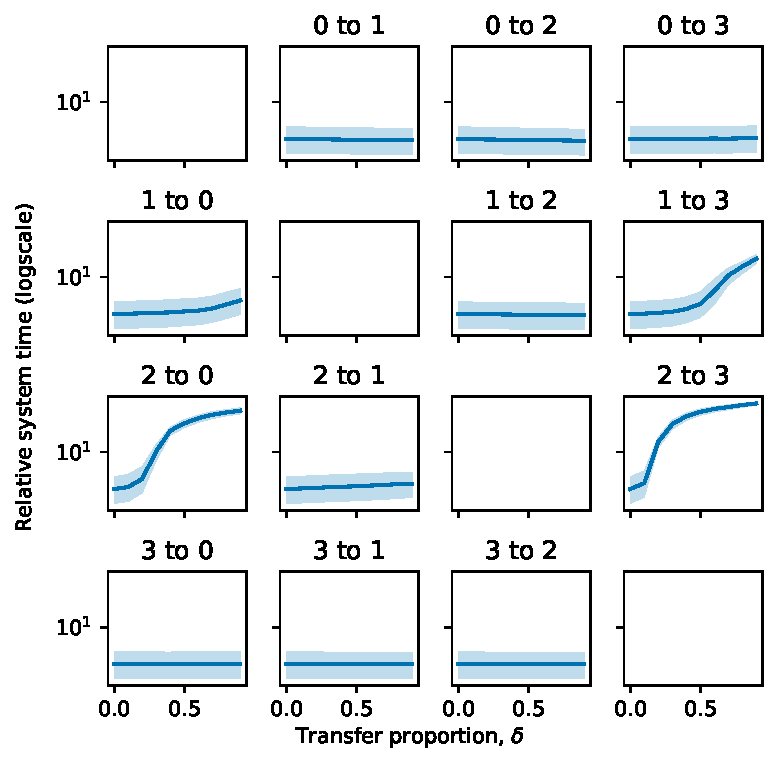
\includegraphics[width=\imgwidth]{moving_time}
    \caption{%
        Plots of proportions of each cluster moving to another against relative
        system time.
    }\label{fig:moving_time}
\end{figure}

\begin{figure}
    \centering
    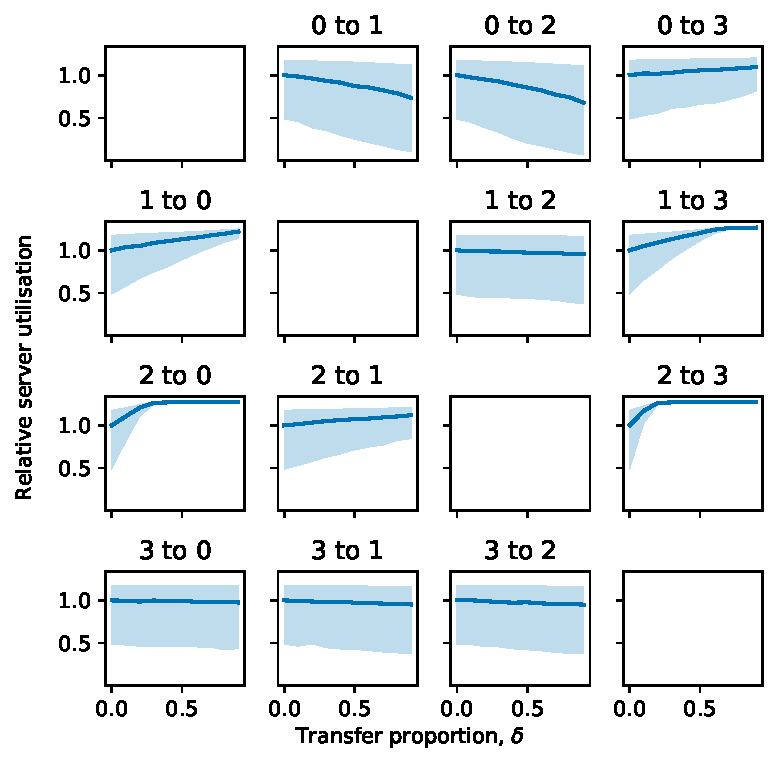
\includegraphics[width=\imgwidth]{moving_utilisation}
    \caption{%
        Plots of proportions of each cluster moving to another on relative mean
        server utilisation.
    }\label{fig:moving_utilisation}
\end{figure}
